% !TEX enableShellEscape = yes
% (The above line makes atom's latex package compile with -shell-escape
% for minted, and is just ignored by other systems.)
\documentclass{article}

\usepackage{fullpage}
\usepackage{color}
\usepackage{amsmath,amssymb}
\usepackage{url}
\usepackage{verbatim}
\usepackage{graphicx}
\usepackage{parskip}
\usepackage{amssymb}
\usepackage{hyperref}

% Use one or the other of these for displaying code.
% NOTE: If you get
%  ! Package minted Error: You must invoke LaTeX with the -shell-escape flag.
% and don't want to use minted, just comment out the next line
\usepackage{minted} \BeforeBeginEnvironment{minted}{\begingroup\color{black}} \AfterEndEnvironment{minted}{\endgroup} \setminted{autogobble,breaklines,breakanywhere,linenos}

\usepackage{listings}

% Colours
\definecolor{blu}{rgb}{0,0,1}
\newcommand{\blu}[1]{{\textcolor{blu}{#1}}}
\definecolor{gre}{rgb}{0,.5,0}
\newcommand{\gre}[1]{\textcolor{gre}{#1}}
\definecolor{red}{rgb}{1,0,0}
\newcommand{\red}[1]{\textcolor{red}{#1}}
\definecolor{pointscolour}{rgb}{0.6,0.3,0}

% answer commands
\newcommand\ans[1]{\par\gre{Answer: #1}}
\newenvironment{answer}{\par\begingroup\color{gre}Answer: }{\endgroup}
\let\ask\blu
\let\update\red
\newenvironment{asking}{\begingroup\color{blu}}{\endgroup}
\newcommand\pts[1]{\textcolor{pointscolour}{[#1~points]}}

% Math
\def\R{\mathbb{R}}
\DeclareMathOperator*{\argmax}{arg\,max}
\DeclareMathOperator*{\argmin}{arg\,min}
\newcommand{\norm}[1]{\lVert #1 \rVert}
\newcommand{\mat}[1]{\begin{bmatrix}#1\end{bmatrix}}

% LaTeX
\newcommand{\fig}[2]{\includegraphics[width=#1\textwidth]{#2}}
\newcommand{\centerfig}[2]{\begin{center}\includegraphics[width=#1\textwidth]{#2}\end{center}}


\begin{document}
    \title{CPSC 340 Assignment 2 (see course page for due date)}
    \author{}
    \date{}
    \maketitle
    \vspace{-4em}


    \section*{Important: Submission Format \pts{5}}

    Please make sure to follow the submission instructions posted on the course website.
    \ask{We will deduct marks if the submission format is incorrect, or if you're not using \LaTeX{} and your handwriting is \emph{at all} difficult to read} -- at least these 5 points, more for egregious issues.
    Compared to assignment 1, your name and student number are no longer necessary (though it's not a bad idea to include them just in case, especially if you're doing the assignment with a partner).


    \section{K-Nearest Neighbours \pts{15}}

    In the \emph{citiesSmall} dataset, nearby points tend to receive the same class label because they are part of the same U.S. state. For this problem, perhaps a $k$-nearest neighbours classifier might be a better choice than a decision tree. The file \emph{knn.py} has implemented the training function for a $k$-nearest neighbour classifier (which is to just memorize the data).

    Fill in the \texttt{predict} function in \texttt{knn.py} so that the model file implements the $k$-nearest neighbour prediction rule.
    You should use Euclidean distance, and may find numpy's \texttt{sort} and/or \texttt{argsort} functions useful.
    You can also use \texttt{utils.euclidean\string_dist\string_squared}, which computes the squared Euclidean distances between all pairs of points in two matrices.
    \begin{enumerate}
        \item Write the \texttt{predict} function. \ask{Submit this code.} \pts{5}
        \begin{minted}{python}
        def predict(self, X_hat):
            n,d = X_hat.shape
            y_hat = np.zeros(n)

            dist = euclidean_dist_squared(self.X, X_hat)
        
            for i in range(n):
                dist_x_hat_i = dist[:,i]
                order = np.argsort(dist_x_hat_i)
                select = order[:self.k]
                KNN_i = self.y[select]
                y_hat[i] = utils.mode(KNN_i)
            return y_hat

        \end{minted}
        
        \item \ask{Report the training and test error} obtained on the \emph{citiesSmall} dataset for $k=1$, $k=3$, and $k=10$. \emph{Optionally}, try running a decision tree on this same train/test split; which gets better test accuracy? \pts{4}
        \begin{table}[!htbp]
            \centering
            \begin{tabular}{ccc}
                \hline
                K & Training Err & Testing Err\\
                \hline
                1 & 0.00 & 0.065\\
                3 & 0.028 & 0.066\\
                10 & 0.072 & 0.097\\
                \hline
            \end{tabular}
        \end{table}
        \item Generate a plot with \texttt{utils.plot\_classifier} on the \emph{citiesSmall} dataset (plotting the training points) for $k=1$, using your implementation of kNN. \ask{Include the plot here.} To see if your implementation makes sense, you might want to check against the plot using \texttt{sklearn.neighbors.KNeighborsClassifier}. Remember that the assignment 1 code had examples of plotting with this function and saving the result, if that would be helpful. \pts{2}
        \begin{figure}[!htbp]
            \centering
            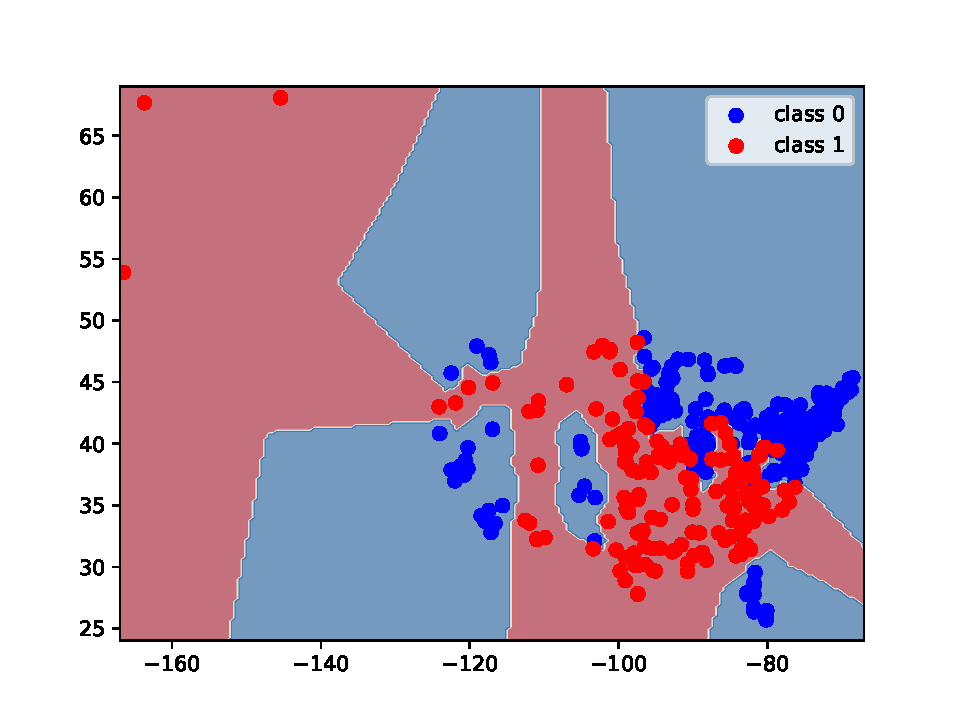
\includegraphics[width = 0.9 \textwidth]{figs/knnDecisionBoundary.pdf}
        \end{figure}

        \item Why is the training error $0$ for $k=1$? \pts{2}
        \begin{answer}
            It's 0 because the algorithm remembers all the classifications of the training data, so it can correctly classify them.
        \end{answer}
        
        \item Recall that we want to choose hyper-parameters so that the test error is (hopefully) minimized. How would you choose $k$? \pts{2}
        
        \begin{answer}
            In this case, we can see that when $K = 1$, we obtain the lowest training error and lowest error, so we should select $K = 1$.

            However, in general, it might not be the case. If we select $K = 1$, then the algorithm would predict exactly based on the training data. So if the test data doesn't have the exact distribution as the training data, we would have a large testing error. However, if we have $K$ to be too large, it would just predict based on the mode of the sample. In practice, we may need to run several times with different $K$ to pick the best one.
        \end{answer}
    \end{enumerate}

    \clearpage
    \section{Picking $k$ in kNN \pts{15}}
    The file \texttt{data/ccdata.pkl} contains a subset of \href{https://www23.statcan.gc.ca/imdb/p2SV.pl?Function=getSurvey&SDDS=2620}{Statistics Canada's 2019 Survey of Financial Security}; we're predicting whether a family regularly carries credit card debt, based on a bunch of demographic and financial information about them. (You might imagine social science researchers wanting to do something like this if they don't have debt information available -- or various companies wanting to do it for less altruistic reasons.) If you're curious what the features are, you can look at the \texttt{'feat\_descs'} entry in the dataset dictionary.

    Anyway, now that we have our kNN algorithm working,\footnote{If you haven't finished the code for question 1, or if you'd just prefer a slightly faster implementation, you can use scikit-learn's \texttt{KNeighborsClassifier} instead. The \texttt{fit} and \texttt{predict} methods are the same; the only difference for our purposes is that \texttt{KNN(k=3)} becomes \texttt{KNeighborsClassifier(n\_neighbors=3)}.} let's try choosing $k$ on this data!

    \begin{enumerate}
        \item Remember the golden rule: we don't want to look at the test data when we're picking $k$. Inside the \texttt{q2()} function of \texttt{main.py}, implement 10-fold cross-validation, evaluating on the \texttt{ks} set there (1, 5, 9, \dots, 29), and store the \emph{mean} accuracy across folds for each $k$ into a variable named \texttt{cv\_accs}.

        Specifically, make sure you test on the first 10\% of the data after training on the remaining 90\%, then test on 10\% to 20\% and train on the remainder, etc -- don't shuffle (so your results are consistent with ours; the data is already in random order). Implement this yourself, don't use scikit-learn or any other existing implementation of splitting. There are lots of ways you could do this, but one reasonably convenient way is to create a \href{https://numpy.org/doc/stable/user/basics.indexing.html#boolean-or-mask-index-arrays}{numpy ``mask'' array}, maybe using \texttt{np.ones(n, dtype=bool)} for an all-\texttt{True} array of length \texttt{n}, and then setting the relevant entries to \texttt{False}. It also might be helpful to know that \texttt{\textasciitilde ary} flips a boolean array (\texttt{True} to \texttt{False} and vice-versa).

        \ask{Submit this code}, following the general submission instructions to include your code in your results file. \pts{5}

        \begin{minted}{python}
        def q2():
            dataset = load_dataset("ccdebt.pkl")
            X = dataset["X"]
            y = dataset["y"]
            X_test = dataset["Xtest"]
            y_test = dataset["ytest"]
            n,d = X.shape

            ks = list(range(1, 30, 4))
            train = np.zeros((8,10))
            test = np.zeros((8,10))
            result = np.zeros((8,4))

            for  a in range(1,9,1):
                k_i = (a - 1) * 4 + 1 
                result[a-1,0] = k_i
                
                #Compute testing error
                model = KNN(k = k_i)
                model.fit(X, y)
                y_hat = model.predict(X_test)
                err = np.mean(y_test != y_hat)
                result[a-1,3] = err

                #Compute errors with cross-validation
                for b in range(1,11,1):
                    low = int(0.1*(b-1)*n)
                    high = int(0.1*b*n)

                    #Generate Mask Array
                    mask = np.ones(n, dtype=bool)
                    mask[i:i+40] = False

                    #Use Mask to Select Data
                    X_test_i = X[~mask,:]
                    y_test_i = y[~mask]
                    X_i = X[mask,:]
                    y_i = y[mask]

                    #Compute Errors
                    model = KNN(k = k_i)

                    #Compute train error
                    model.fit(X_i, y_i)
                    y_hat = model.predict(X_i)
                    err_train = np.mean(y_i != y_hat)
                    train[a-1,b-1] = err_train
                    
                    # Compute test error
                    y_hat_test = model.predict(X_test_i)
                    err_test = np.mean(y_hat_test != y_test_i)
                    test[a-1,b-1] = err_test


                result[a-1, 1] = np.mean(train[a-1,:])
                result[a-1, 2] = np.mean(test[a-1,:])
            cv_accs = result[:,2]

        \end{minted}

        

        \item The point of cross-validation is to get a sense of what the test error for a particular value of $k$ would be. Implement, similarly to the code you wrote for question 1.2, a loop to compute the test accuracy for each value of $k$ above. \ask{Submit a plot the cross-validation and test accuracies as a function of $k$.} Make sure your plot has axis labels and a legend. \pts{5}
        \begin{answer}
            Check \hyperref[fig2.2]{Figure 2.2}
        \end{answer}

        \begin{figure}[!htbp]
            \label{fig2.2}
            \centering
            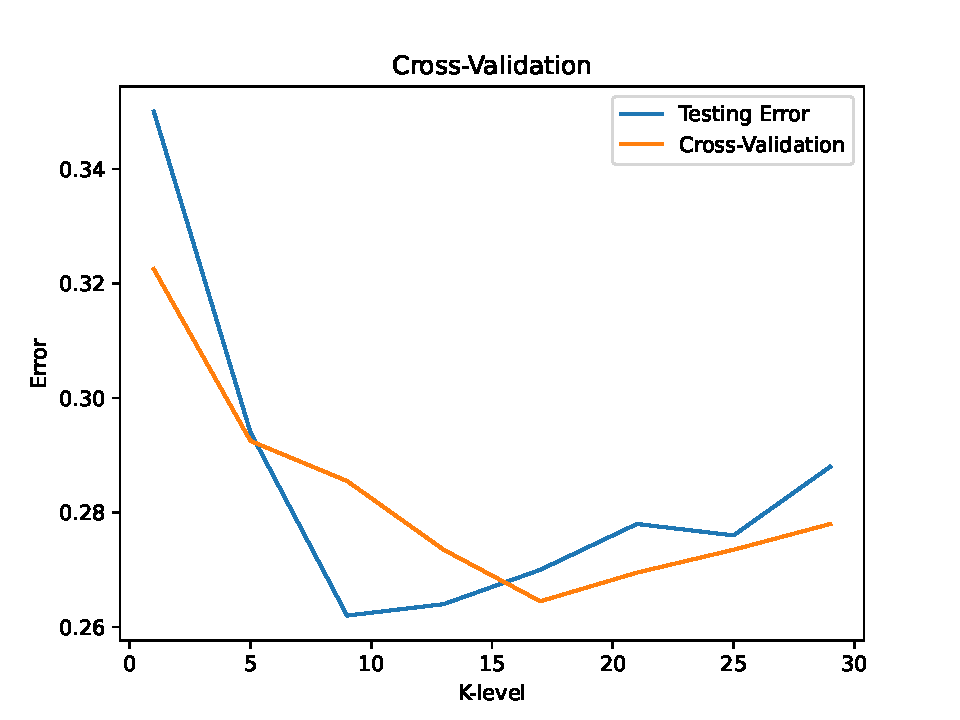
\includegraphics[width = 0.8\textwidth]{figs/Cross-Validation.pdf}
            \caption{Figure 2.2}
        \end{figure}

        \item Which $k$ would cross-validation choose in this case? Which $k$ has the best test accuracy? Would the cross-validation $k$ do okay (qualitatively) in terms of test accuracy? \pts{2}
        
        \begin{answer}
            Cross-validation would pick $K = 17$. It also gives us a relatively low testing error, though not the lowert.
        \end{answer}

        %

        \item Separately, \ask{submit a plot of the training error as a function of $k$. How would the $k$ with best training error do in terms of test error, qualitatively?} \pts{3}
        \begin{answer}
            Check \hyperref[fig2.4]{Figure 2.4}
        \end{answer}
        
        \begin{figure}[!htbp]
            \label{fig2.4}
            \centering
            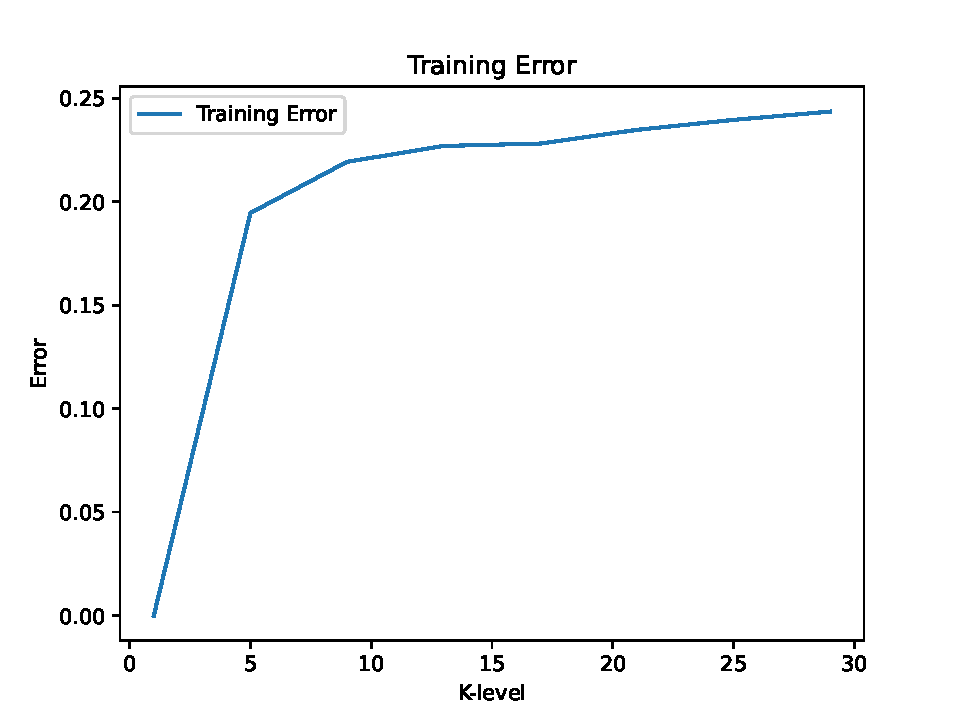
\includegraphics[width = 0.8\textwidth]{figs/TrainingError.pdf}
            \caption{Figure 2.4}
        \end{figure}
        %
    \end{enumerate}



    \clearpage
    \section{Na\"ive Bayes \pts{17}}

    In this section we'll implement Na\"ive Bayes, a very fast classification method that is often surprisingly accurate for text data with simple representations like bag of words.


    \subsection{Na\"ive Bayes by Hand \pts{5}}

    Consider the dataset below, which has $10$ training examples and $3$ features:
    \[
    X = \begin{bmatrix}
        0 & 0 & 1\\
        0 & 1 & 1\\
        0 & 1 & 1\\
        1 & 1 & 0\\
        0 & 1 & 0\\
        0 & 1 & 1\\
        0 & 1 & 0\\
        1 & 1 & 0\\
        1 & 0 & 0\\
        0 & 0 & 0
    \end{bmatrix},
    \quad y = \begin{bmatrix}
        \text{spam}\\
        \text{spam}\\
        \text{spam}\\
        \text{spam}\\
        \text{spam}\\
        \text{spam}\\
        \text{not spam}\\
        \text{not spam}\\
        \text{not spam}\\
        \text{not spam}
    \end{bmatrix}.
    \]
    The feature in the first column is $<$your name$>$ (whether the e-mail contained your name), in the second column is ``lottery'' (whether the e-mail contained this word), and the third column is ``Venmo'' (whether the e-mail contained this word).
    Suppose you believe that a naive Bayes model would be appropriate for this dataset, and you want to classify the following test example:
    \[
    \hat{x} = \begin{bmatrix}1 & 1 & 0\end{bmatrix}.
    \]

    \subsubsection{Prior probabilities \pts{1}}
    \ask{Compute the estimates of the class prior probabilities, which I also called the ``baseline spam-ness'' in class.} (you don't need to show any work):
    \begin{itemize}
        \item $\Pr(\text{spam})$.
        \begin{answer}
            $60\%$
        \end{answer}
        \item $\Pr(\text{not spam})$.
        \begin{answer}
            $40\%$
        \end{answer}
    \end{itemize}

    \subsubsection{Conditional probabilities \pts{1}}

    \ask{Compute the estimates of the 6 conditional probabilities required by Na\"ive Bayes for this example}  (you don't need to show any work):
    \begin{itemize}
        \item $\Pr(\text{$<$your name$>$} = 1  \mid \text{spam})$.
        \begin{answer}
            $\frac{1}{6}$
        \end{answer}
    
        \item $\Pr(\text{lottery} = 1 \mid \text{spam})$.
        \begin{answer}
            $\frac{5}{6}$
        \end{answer}
        \item $\Pr(\text{Venmo} = 0  \mid \text{spam})$.
        \begin{answer}
            $\frac{2}{3}$
        \end{answer}
        \item $\Pr(\text{$<$your name$>$} = 1  \mid \text{not spam})$.
        \begin{answer}
            $\frac{1}{2}$
        \end{answer}
        \item $\Pr(\text{lottery} = 1  \mid \text{not spam})$.
        \begin{answer}
            $\frac{1}{2}$
        \end{answer}
        \item $\Pr(\text{Venmo} = 0  \mid \text{not spam})$.
        \begin{answer}
            1
        \end{answer}
        %
    \end{itemize}

    \subsubsection{Prediction \pts{2}}


    \ask{Under the naive Bayes model and your estimates of the above probabilities, what is the most likely label for the test example? \textbf{(Show your work.)}}
    \begin{answer}
        Assuming all the X's are independent, we have
        \begin{equation}
            P(\hat{y} = 1 | \hat{x}) \propto \prod_{i = 1}^3 P(\hat{x_{i}}| \hat{y} = 1) P(\hat{y} = 1) = \frac{1}{50}
        \end{equation}

        On the other hand,
        \begin{equation}
            P(\hat{y} = 0 | \hat{x})  \propto \prod_{i = 1}^3 P(\hat{x_{i}}| \hat{y} = 0) P(\hat{y} = 0)= 0
        \end{equation}

        Therefore, we have,
        \begin{equation}
            P(\hat{y} = 1 | \hat{x}) > P(\hat{y} = 0 | \hat{x})
        \end{equation}

        Then $\hat{y} = 1$
    \end{answer}
    %

    \subsubsection{Simulating Laplace Smoothing with Data \pts{1}}
    \label{laplace.conceptual}

    One way to think of Laplace smoothing is that you're augmenting the training set with extra counts. Consider the estimates of the conditional probabilities in this dataset when we use Laplace smoothing (with $\beta = 1$).
    \ask{Give a set of extra training examples where, if they were included in the training set, the ``plain'' estimation method (with no Laplace smoothing) would give the same estimates of the conditional probabilities as using the original dataset with Laplace smoothing.}
    Present your answer in a reasonably easy-to-read format, for example the same format as the data set at the start of this question.

    \begin{answer}
        We can add an extra data set $X'$ and $y'$, such that 
        \[
            X' = \begin{bmatrix}
            1&1&1 \\
            0&0&0 \\
            1&1&1 \\
            0&0&0 \\
        \end{bmatrix}
        ,\quad
        y' = \begin{bmatrix}
            spam\\
            spam\\
            not spam\\
            not spam\\
        \end{bmatrix}
        \]
    \end{answer}

    \subsection{Exploring Bag-of-Words \pts{2}}

    If you run \texttt{python main.py 3.2}, it will load the following dataset:
    \begin{enumerate}
        \item \texttt{X}: A binary matrix. Each row corresponds to a newsgroup post, and each column corresponds to whether a particular word was used in the post. A value of $1$ means that the word occured in the post.
        \item \texttt{wordlist}: The set of words that correspond to each column.
        \item \texttt{y}: A vector with values $0$ through $3$, with the value corresponding to the newsgroup that the post came from.
        \item \texttt{groupnames}: The names of the four newsgroups.
        \item \texttt{Xvalidate} and \texttt{yvalidate}: the word lists and newsgroup labels for additional newsgroup posts.
    \end{enumerate}
    \ask{Answer the following}:
    \begin{enumerate}
        \item Which word corresponds to column 73 of $X$? (This is index 72 in Python.)
        \begin{answer}
            'question'
        \end{answer}
        \item Which words are present in training example 803 (Python index 802)?
        \begin{answer}
            'case' 'children' 'health' 'help' 'problem' 'program'
        \end{answer}
        \item Which newsgroup name does training example 803 come from?
        \begin{answer}
            3
        \end{answer}
        %
    \end{enumerate}

    \subsection{Na\"ive Bayes Implementation \pts{4}}

    If you run \texttt{python main.py 3.3}
    it will load the newsgroups dataset, fit a basic naive Bayes model and report the validation error.

    The \texttt{predict()} function of the naive Bayes classifier is already implemented.
    However, in \texttt{fit()}
    the calculation of the variable \texttt{p\_xy} is incorrect
    (right now, it just sets all values to $1/2$).
    \ask{Modify this function so that \texttt{p\_xy} correctly
        computes the conditional probabilities of these values based on the
        frequencies in the data set. Submit your code. Report the training and validation errors that you obtain.}
    \begin{answer}
        The training error is 0.200, and the validation error is 0.188.

        The code is as following:
    \end{answer}


    \begin{minted}{python}
        def fit(self, X, y):
            n, d = X.shape

            # Compute the number of class labels
            k = self.num_classes

            # Compute the probability of y
            counts = np.bincount(y)
            p_y = counts / n

            #Compute the conditional probabilities 
            p_xy = np.zeros((d,k))
            for j in range(k):
                mask_j = np.where(y == j , True , False)
                X_j = X[mask_j]
                for i in range(d):
                    p_xy[i,j] = np.mean(X_j[:,i]) 

            self.p_y = p_y
            self.p_xy = p_xy
    \end{minted}
    


    \subsection{Laplace Smoothing Implementation \pts{4}}

    Laplace smoothing is one way to prevent failure cases of Na\"ive Bayes based on counting. Recall what you know from lecture to implement Laplace smoothing to your Na\"ive Bayes model.
    \begin{itemize}
        \item Modify the \texttt{NaiveBayesLaplace} class provided in \texttt{naive\_bayes.py} and write its \texttt{fit()} method to implement Laplace smoothing. \ask{Submit this code.}
        \begin{minted}{python}
        def fit(self, X, y, beta):
            n, d = X.shape

            # Compute the number of class labels
            k = self.num_classes

            # Compute the probability of y
            counts = np.bincount(y)
            p_y = counts / n

            #Compute the conditional probabilities 
            p_xy = np.zeros((d,k))
            for j in range(k):
                mask_j = np.where(y == j , True , False)
                X_j = X[mask_j]
                for i in range(d):
                    p_xy[i,j] = (np.count_nonzero(X_j[:,i]) + beta)/(X_j.shape[0] + *beta)
            print(p_xy[:,0])

            self.p_y = p_y
            self.p_xy = p_xy
        \end{minted}
        
        \item Using the same data as the previous section, fit Na\"ive Bayes models with \textbf{and} without Laplace smoothing to the training data. Use $\beta=1$ for Laplace smoothing. For each model, look at $p(x_{ij} = 1 \ | \ y_i = 0)$ across all $j$ values (i.e. all features) in both models. \ask{Do you notice any difference? Explain.}
        \begin{answer}
            Without the Laplace smoothing, we have 12 zero entries in the conditional probabilities matrixs, which is problematice when we predict. After the Laplace smoothing, we have none zero entries.
        \end{answer}
        \item One more time, fit a Na\"ive Bayes model with Laplace smoothing using $\beta=10000$. Look at $p(x_{ij} = 1 \ | \ y_i = 0)$. \ask{Do these numbers look like what you expect? Explain.}
        \begin{answer}
            All the numbers are close to 0.25. Since we add 10000 in the numerators and 20000 in the denominator, which are too large to our sample size(8121). So all the conditional probabilities will be driven close to $1/K$, and in this case we have $1/K = 1/4$.
        \end{answer}
        %
    \end{itemize}

    \subsection{Runtime of Na\"ive Bayes for Discrete Data \pts{2}}

    For a given training example $i$, the predict function in the provided code computes the quantity
    \[
    p(y_i \mid x_i) \propto p(y_i)\prod_{j=1}^d p(x_{ij} \mid y_i),
    \]
    for each class $y_i$ (and where the proportionality constant is not relevant). For many problems, a lot of the $p(x_{ij} \mid y_i)$ values may be very small. This can cause the above product to underflow. The standard fix for this is to compute the logarithm of this quantity and use that $\log(ab) = \log(a)+\log(b)$,
    \[
    \log p(y_i \mid x_i) = \log p(y_i) + \sum_{j=1}^d \log p(x_{ij} \mid y_i) + \text{(log of the irrelevant proportionality constant)} \, .
    \]
    This turns the multiplications into additions and thus typically would not underflow.
    % XXX this is true, but not super relevant to the rest of the question,
    %     which is kind of confusing to students...

    Assume you have the following setup:
    \begin{itemize}
        \item The training set has $n$ objects each with $d$ features.
        \item The test set has $t$ objects with $d$ features.
        \item Each feature can have up to $c$ discrete values (you can assume $c \leq n$).
        \item There are $k$ class labels (you can assume $k \leq n$).
    \end{itemize}
    You can implement the training phase of a naive Bayes classifier in this setup in $O(\update{k c d + {}} nd)$, since you only need to do a constant amount of work for each $x_{ij}$ value\update{; usually $k c \ll n$ and so this is $O(n d)$}. (You do not have to actually implement it in this way for the previous question, but you should think about how this could be done.)
    \ask{What is the cost of classifying $t$ test examples with the model and this way of computing the predictions?}
    \update{It's preferable to leave your answer in terms of $k$ and $c$ if relevant.}
    \begin{answer}
        For each of the \textcolor{red}{t} entries, we need to calculate \textcolor{red}{k} different conditional probabilities to compare. Within each calculation, we have \textcolor{red}{d} items to product. Therefore, all together, the computational cost would be \textcolor{red}{O(tkd)}
    \end{answer}
    %


    \clearpage
    \section{Random Forests \pts{15}}

    The file \texttt{vowels.pkl} contains a supervised learning dataset where we are trying to predict which of the 11 ``steady-state'' English vowels that a speaker is trying to pronounce.

    You are provided with a \texttt{RandomStump} class that differs from
    \texttt{DecisionStumpInfoGain} in that
    it only considers $\lfloor \sqrt{d} \rfloor$ randomly-chosen features.\footnote{The notation $\lfloor x\rfloor$ means the ``floor'' of $x$, or ``$x$ rounded down''. You can compute this with \texttt{np.floor(x)} or \texttt{math.floor(x)}.}
    You are also provided with a \texttt{RandomTree} class that is exactly the same as
    \texttt{DecisionTree} except that it uses \texttt{RandomStump} instead of
    \texttt{DecisionStump} and it takes a bootstrap sample of the data before fitting.
    In other words, \texttt{RandomTree} is the entity we discussed in class, which
    makes up a random forest.

    If you run \texttt{python main.py 4} it will fit a deep \texttt{DecisionTree}
    using the information gain splitting criterion. You will notice that the model overfits badly.




    \begin{enumerate}
        \item Using the provided code, evaluate the \texttt{RandomTree} model of unlimited depth. \ask{Why doesn't the random tree model have a training error of 0?} \pts{2}
        \begin{answer}
            Because in the \texttt{RandomTree} model, it's trained by the bootstrap data, but compared with the original data. Since the bootstrap data is not identical with the original data, there will be training errors.
        \end{answer}
        \item For \texttt{RandomTree}, if you set the \texttt{max\_depth} value to \texttt{np.inf}, \ask{why do the training functions terminate instead of making an infinite number of splitting rules?} \pts{2}
        \begin{answer}
            Though we set the maximum depth to be infinity, but there is a certain level of depth that any depth beyond that would not change the result of the decision tree. That's where the model stops.
        \end{answer}
        \item Complete the \texttt{RandomForest} class in \texttt{random\string_tree.py}. This class takes in hyperparameters \texttt{num\string_trees} and \texttt{max\string_depth} and
        fits \texttt{num\string_trees} random trees each with maximum depth \texttt{max\string_depth}. For prediction, have all trees predict and then take the mode. \ask{Submit this code.} \pts{5}
        \begin{minted}{python}
        class RandomForest:
            def __init__(self, max_depth, num_trees):
                DecisionTree.__init__(
                    self, max_depth=max_depth, stump_class=RandomStumpInfoGain
                )
                self.num_trees = num_trees

            def fit(self, X, y):
                #For simplicity, store 50 tree models
                self.trees = []
                for i in range(self.num_trees):
                    tree = RandomTree(max_depth=self.max_depth)
                    tree.fit(X, y)
                    self.trees.append(tree)
                    
            def predict(self, X):
                n = X.shape[0]
                y = np.zeros(n)

                #Generate a result matrix
                result = np.zeros((n, self.num_trees))

                #For each tree, generate a prediction vector, store it in a matrix
                for i, tree in enumerate(self.trees):
                    y_i  = tree.predict( X)
                    result[:,i] = y_i

                #Find the mode of the predictions
                for i in range(n):
                    y[i] = utils.mode(result[i,:])

                return y
        \end{minted}
        \item Using 50 trees, and a max depth of $\infty$, \ask{report the training and testing error}. Compare this to what we got with a single \texttt{DecisionTree} and with a single \texttt{RandomTree}. \ask{Are the results what you expected? Discuss.} \pts{3}
        \begin{answer}
            The \texttt{RandomTree} model gives us 0 training error and 0.182 testing error. It is the result we expect since it has lower training error than a single random tree and a lower testing error than a single decision tree
        \end{answer}
        \item \ask{Why does a random forest typically have a training error of 0, even though random trees typically have a training error greater than 0?} \pts{3}
        \begin{answer}
            Since even though each random tree use different bootstrap data, they are very familiar with the original data. Therefore, when we use a random forest with a lot of random trees, the mode of their perdiction will be the same as we trained from 
        \end{answer}
        %
    \end{enumerate}


    \clearpage
    \section{Clustering \pts{15}}

    If you run \verb|python main.py 5|, it will load a dataset with two features
    and a very obvious clustering structure. It will then apply the $k$-means algorithm
    with a random initialization. The result of applying the
    algorithm will thus depend on the randomization, but a typical run might look like this:
    \centerfig{.5}{figs/kmeans_basic.png}
    (Note that the colours are arbitrary -- this is the label switching issue.)
    But the ``correct'' clustering (that was used to make the data) is this:
    \centerfig{.5}{figs/kmeans_good.png}


    \subsection{Selecting among $k$-means Initializations \pts{7}}

    If you run the demo several times, it will find different clusterings. To select among clusterings for a \emph{fixed} value of $k$, one strategy is to minimize the sum of squared distances between examples $x_i$ and their means $w_{y_i}$,
    \[
    f(w_1,w_2,\dots,w_k,y_1,y_2,\dots,y_n) = \sum_{i=1}^n \norm{x_i - w_{y_i}}_2^2 = \sum_{i=1}^n \sum_{j=1}^d (x_{ij} - w_{y_ij})^2.
    \]
    where $y_i$ is the index of the closest mean to $x_i$. This is a natural criterion because the steps of $k$-means alternately optimize this objective function in terms of the $w_c$ and the $y_i$ values.

    \begin{enumerate}
        \item In the \texttt{kmeans.py} file, complete the \texttt{error()} method. \texttt{error()} takes as input the data used in fit (\texttt{X}), the indices of each examples' nearest mean (\texttt{y}), and the current value of means (\texttt{means}). It returns the value of this above objective function. \ask{Submit this code. What trend do you observe if you print the value of this error after each iteration of the $k$-means algorithm?} \pts{4}
        \begin{answer}
            After each iteration, the error is lowered
        \end{answer}
        \begin{minted}{python}
            def error(self, X, y, means):
                n = X.shape[0]
                err = np.int(0)
                for i in range(n):
                    err += np.sum((X[i,:] - means[y[i],:]) ** 2)
                return err
        \end{minted}
        \item Run $k$-means 50 times (with $k=4$) and take the one with the lowest error. \ask{Report the lowest error obtained.} Visualize the clustering obtained by this model, and \ask{submit your plot}. \pts{3}
        \begin{answer}
            The lowest error I got is 3071. We can see from figure~\ref{fig5.1.2} that the error of each time seems to be random within 3 steady states. Since each time the k-mean algorithm would update untill the categorises are steady, we could have 3 different ways of steady classification. 
        \end{answer}
        \begin{figure}
            \centering\label{fig5.1.2}
            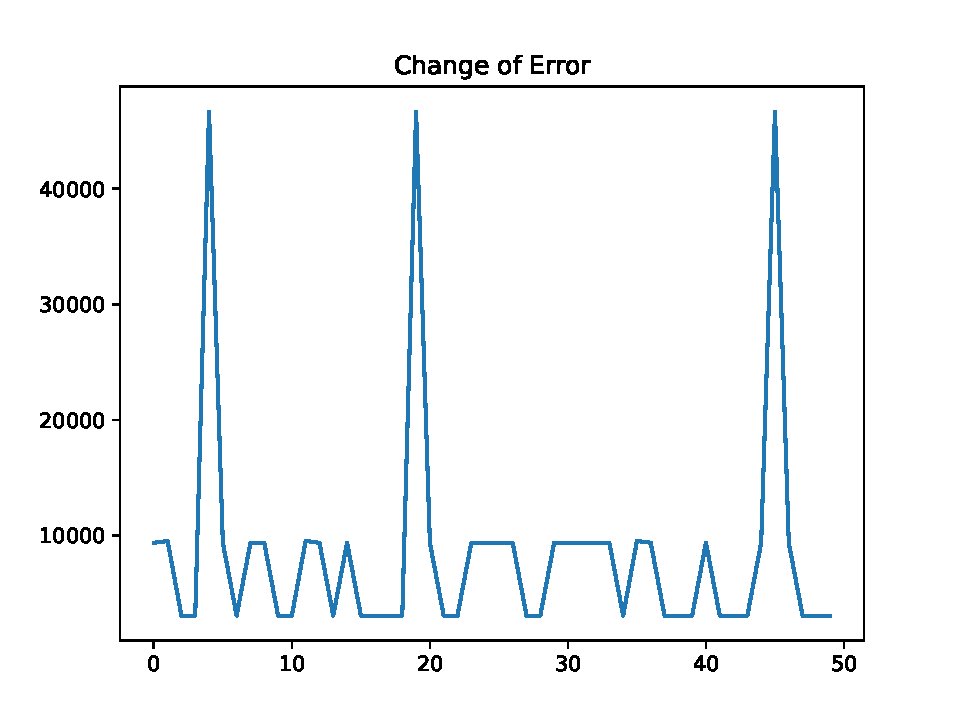
\includegraphics[width = 0.8\textwidth]{figs/kmeans_error.pdf}
        \end{figure}
    \end{enumerate}


    \subsection{Selecting $k$ in $k$-means \pts{8}}

    We now turn to the task of choosing the number of clusters $k$.

    \begin{enumerate}
        \item \ask{Explain why we should not choose $k$ by taking the value that minimizes the \texttt{error} value.} \pts{2}
        \begin{answer}
            We could pick a very large k that minimize the error. For example, if we have k equal to our sample size, then we could potential have 0 error. But that doesn't give us a meaningful classification.
        \end{answer}
        %
        \item \ask{Is evaluating the \texttt{error} function on \update{validation (or} test\update{)} data a suitable approach to choosing $k$?} \pts{2}
        \begin{answer}
            First of all, no matter what data we are working on, a larger k would always result in a smaller error. Secondly, this is a unsupervised learning, and we don't have a real y to compare with during the training period. Therefore, the error won't be different if we are using test data or not.
        \end{answer}
        \item \ask{Hand in a plot of the minimum error found across 50 random initializations, as a function of $k$, taking $k$ from $1$ to $10$.} \pts{2}
        \begin{answer}
            See figure~\ref{fig5.2.3}
        \end{answer}
        \begin{figure}
            \centering\label{fig5.2.3}
            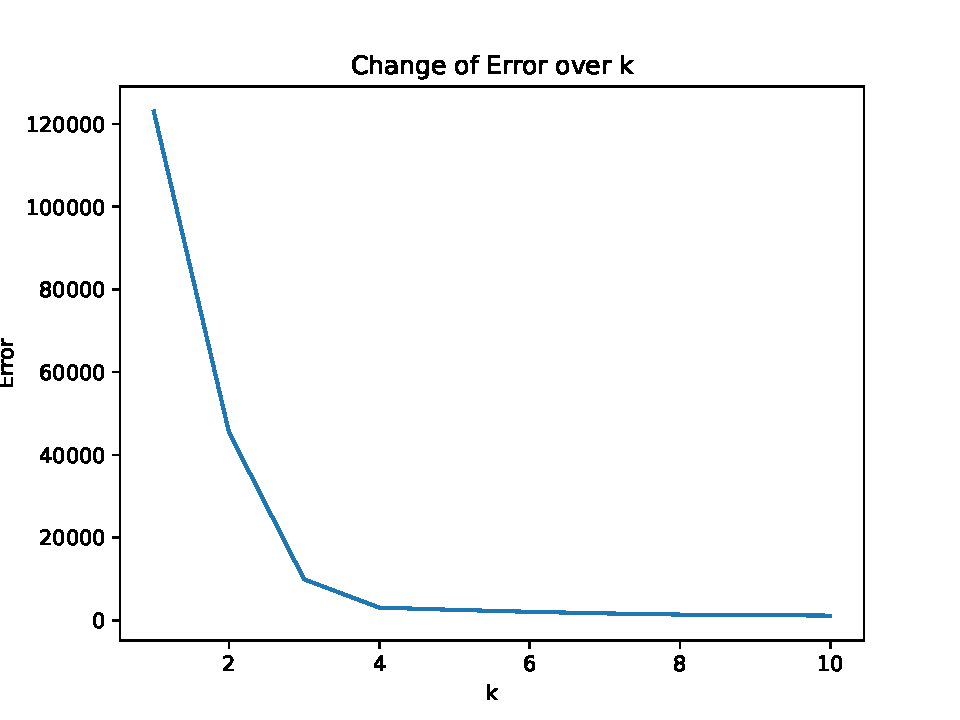
\includegraphics[width = .8\textwidth]{figs/k_selection.pdf}
        \end{figure}
        %
        \item The \emph{elbow method} for choosing $k$ consists of looking at the above plot and visually trying to choose the $k$ that makes the sharpest ``elbow" (the biggest change in slope). \ask{What values of $k$ might be reasonable according to this method?} Note: there is not a single correct answer here; it is somewhat open to interpretation and there is a range of reasonable answers. \pts{2}
        \begin{answer}
            Without calculating the real slope, the selection of $k = 3$ and $k = 4$ both seems plausible.
        \end{answer}
    \end{enumerate}

    \clearpage
    \section{Very-Short Answer Questions \pts{18}}

    \ask{Write a short one or two sentence answer to each of the questions below}. Make sure your answer is clear and concise.

  



    \begin{enumerate}
        \item What is a reason that the the data may not be IID in the email spam filtering example from lecture?
        \begin{answer}
            If one register on a shopping website, and then several brands send him spam email because of that, then the data of his email is not IID.
        \end{answer}
        
        \item Why can't we (typically) use the training error to select a hyper-parameter?
        \begin{answer}
            Because what we want from the algorithm it to accrately test/classify new data. However, training error can only shows how well the algorithm learns from the training data. If we select hyper-parameter by training error, we could always have a model that remembers and always reports the true output. However, it's useless. This problem can also be generalized as overfitting problem.
        \end{answer}

        \item What is the effect of the training or validation set size $n$ on the optimization bias, assuming we use a parametric model?
        \begin{answer}
            As $n$ increase, the bias would decrease. However, there would be a lowest bias that can't be eliminate by parametric model.
        \end{answer}

        \item What is an advantage and a disadvantage of using a large $k$ value in $k$-fold cross-validation?
        \begin{answer}
            With $k$ large, we would have more data when fitting the model. However, at the same time, we need to fit more models.
        \end{answer}

        \item Recall that false positive in binary classification means $\hat y_i=1$ while $\tilde y_i = 0$. Give an example of when increasing false positives is an acceptable risk.
        \begin{answer}
            When testing for cancer or any kind of deadly disease, a false positive would be much more acceptable than a false negative.
        \end{answer}

        \item Why can we ignore $p(x_i)$ when we use naive Bayes?
        \begin{answer}
            Firstly, it won't affect the relative relationship between different $p(y_i = c | x_i)$. Secondly, it can sometimes be zero and meaningless.
        \end{answer}

        \item For each of the three values below in a naive Bayes model, say whether it's better considered as a parameter or a hyper-parameter:
        \begin{enumerate}
            \item Our estimate of $p(y_i)$ for some $y_i$.
            \begin{answer}
                Parameter. It's learned from sample.
            \end{answer}
            \item Our estimate of $p(x_{ij} \mid y_i)$ for some $x_{ij}$ and $y_i$.
            \begin{answer}
                Parameter. It's learned from sample.
            \end{answer}
            \item The value $\beta$ in Laplace smoothing.
            \begin{answer}
                Hyper-parameter. Since it's set previously.
            \end{answer}
        \end{enumerate}
        %

        \item Both supervised learning and clustering models take in an input $x_i$ and produce a label $y_i$. What is the key difference between these types of models?
        \begin{answer}
            In supervised learning, we will compare our result with the true $y$ to improve the accuracy during the training. However, we don't have it in the clustering model(unsupervised learning).
        \end{answer}

        \item In $k$-means clustering the clusters are guaranteed to be convex regions. Are the areas that are given the same label by kNN also convex?
        \begin{answer}
            No they are not. KNN would find a close neighborhohd and classify based on the mode. It doesn't guarantee the points on the segment connecting two elements in the same category would all be in the same one. 
        \end{answer}
    \end{enumerate}

\end{document}
